\documentclass{article}
\usepackage{style}

\usepackage{url, hyperref}
\usepackage{array}
\usepackage{tabularx}
\usepackage{siunitx}
\usepackage{paralist}
\usepackage[
	style=numeric,
	sorting=none,
	maxbibnames=10]{biblatex}
\addbibresource{ref.bib}
\bibliography{ref.bib}

\begin{document}

% University Logo, Course Name, Professor's Name, Date, Homework Title,
% Homework Number, Student Name, Student Identifier, Source Code
\cover{./UTFPR.png}{Circuitos Elétricos 1}{Juliano Scholz Slongo}{03/05/2025}
{Laboratório}{1}{Gabriel dos Santos Schmitz \& Henrique Acaio de Souza Farias}{2487438 \& 2399040}
{https://github.com/gabrielzschmitz/uni/tree/main/circuitos-1/lab1}

\section{Introdução}

Irei neste documento debruçar-me-ei sobre a Geometria Analítica desde a noção
intuitiva de tratamento geométrico até o produto misto entre vetores. Farei isto
baseando-me nos livros \citetitle{winterle2014vetores}
\cite{winterle2014vetores} e \citetitle{steimbruch1987geometria}
\cite{steimbruch1987geometria}. Conforme a bibliografia usada no curso Geometria
Analítica na UTFPR de Toledo.

\section{Análise Teórica}

Neste experimento, realizamos a análise teórica de um circuito resistivo
utilizando o método da análise nodal. O objetivo é determinar os potenciais
elétricos nos nós principais, as correntes que circulam pelos resistores e as
potências envolvidas no circuito.

\begin{figure}[H]
  \centering
  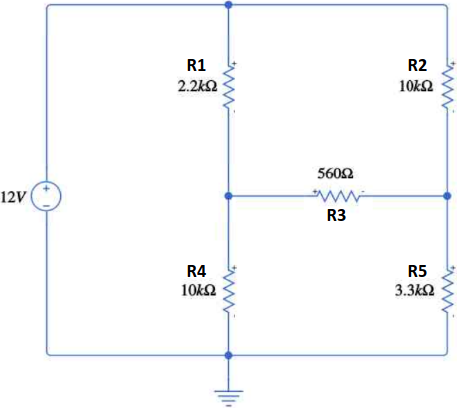
\includegraphics[width=0.5\linewidth]{fig/lab1circuit.png}
  \caption{Circuito para análise em laboratório}
  \label{fig:circuit}
\end{figure}

\subsection{Análise Nodal}

Para determinar as tensões nos nós do circuito, aplicamos a Lei de Kirchhoff das
Correntes (LKC) nos dois principais nós de interesse, denominados \(v_1\) e
\(v_2\). Essa lei estabelece que a soma algébrica das correntes que entram e
saem de um nó é igual a zero.

\begin{itemize}
  \item Nó 1: \(v_1\) (entre R1, R3, R4)
    \[
      \frac{v_1 - 12}{2200} + \frac{v_1 - v_2}{560} + \frac{v_1 - v_2}{10000} = 0
    \]
  \item Nó 2: \(v_2\) (entre R2, R3, R5)
    \[
      \frac{v_2 - 12}{10000} + \frac{v_2 - v_1}{560} + \frac{v_2}{3300} = 0
    \]
\end{itemize}

\subsection{Sistema Linear}

As equações obtidas na análise nodal são reorganizadas para formar um sistema
linear, no qual isolamos os termos relacionados a \(v_1\) e \(v_2\). Isso
facilita a resolução por métodos algébricos.

A seguir, expressamos as equações no formato padrão do sistema:

\[
\left\{
\begin{aligned}
  \left( \frac{1}{2200} + \frac{1}{560} + \frac{1}{10000} \right)v_1 - \left( \frac{1}{560} + \frac{1}{10000} \right)v_2 &= \frac{12}{2200} \\
  - \frac{1}{560}v_1 + \left( \frac{1}{10000} + \frac{1}{560} + \frac{1}{3300} \right)v_2 &= \frac{12}{10000}
\end{aligned}
\right.
\]

Convertendo as frações para valores decimais, obtemos:

\[
\left\{
\begin{aligned}
  0.000988v_1 - 0.001179v_2 &= 0.005455 \\
  -0.001786v_1 + 0.002448v_2 &= 0.0012
\end{aligned}
\right.
\]

Este sistema pode ser resolvido por substituição, método de Gauss ou matriz
inversa. O resultado fornece as tensões nos nós:

\[
  v_1 \approx 7{,}30\,\text{V}, \quad v_2 \approx 6{,}51\,\text{V}
\]

\subsection{Cálculo das Correntes nos Resistores (em mA)}

Com os valores de \(v_1\) e \(v_2\) obtidos, podemos calcular a corrente em cada
resistor usando a Lei de Ohm \(I = \frac{V}{R}\), considerando a queda de tensão
correspondente em cada resistor.

\begin{itemize}
  \item 
    \(I_{R1} = \frac{12 - v_1}{2200} = \frac{4.70}{2200} \approx \SI{2.14}{\milli\ampere}\)
  \item
    \(I_{R2} = \frac{12 - v_2}{10000} = \frac{5.49}{10000} \approx \SI{0.549}{\milli\ampere}\)
  \item
    \(I_{R3} = \frac{v_1 - v_2}{560} = \frac{0.79}{560} \approx \SI{1.41}{\milli\ampere}\)
  \item
    \(I_{R4} = \frac{v_1 - v_2}{10000} = \frac{0.79}{10000} \approx \SI{0.72}{\milli\ampere}\)
  \item
    \(I_{R5} = \frac{v_2 - 0}{3300} = \frac{6.51}{3300} \approx \SI{1.97}{\milli\ampere}\)
\end{itemize}

\subsection{Cálculo das Tensões nos Resistores (em V)}

A tensão sobre cada resistor também pode ser obtida via \(V = R \cdot I\),
confirmando os valores já utilizados no cálculo das correntes.

\begin{itemize}
  \item \(V_{R1} = R_1 \cdot I_{R1} = 2200 \cdot 0.00214 = \SI{4.70}{\volt}\)
  \item \(V_{R2} = 10000 \cdot 0.000549 = \SI{5.49}{\volt}\)
  \item \(V_{R3} = 560 \cdot 0.00141 = \SI{0.79}{\volt}\)
  \item \(V_{R4} = 10000 \cdot 0.000079 = \SI{7.28}{\volt}\)
  \item \(V_{R5} = 3300 \cdot 0.00197 = \SI{6.51}{\volt}\)
\end{itemize}

\subsection{Cálculo da Potência Dissipada por Cada Resistor (em mW)}

A potência dissipada em cada resistor é calculada por \(P = V \cdot I\), sendo
importante para avaliar o consumo energético e a viabilidade dos componentes.

\begin{itemize}
  \item \(P_{R1} = 4.70 \cdot 0.00214 \approx \SI{10.06}{\milli\watt}\)
  \item \(P_{R2} = 5.49 \cdot 0.000549 \approx \SI{3.01}{\milli\watt}\)
  \item \(P_{R3} = 0.79 \cdot 0.00141 \approx \SI{1.11}{\milli\watt}\)
  \item \(P_{R4} = 0.79 \cdot 0.000079 \approx \SI{5.29}{\milli\watt}\)
  \item \(P_{R5} = 6.51 \cdot 0.00197 \approx \SI{12.82}{\milli\watt}\)
\end{itemize}

\subsection{Corrente e Potência da Fonte}

Finalmente, é possível calcular a corrente total fornecida pela fonte somando as
correntes nos ramos diretamente ligados a ela. A potência fornecida é então:

\begin{itemize}
  \item Corrente da fonte: \(I = I_{R1} + I_{R2} = 2.14 + 0.549 = \SI{2.69}{\milli\ampere}\)
  \item Potência fornecida: \(P = V \cdot I = 12 \cdot 0.00269 = \SI{32.28}{\milli\watt}\)
\end{itemize}

Esses resultados permitem validar a consistência do circuito e avaliar se os
componentes estão operando dentro de suas especificações.
\section{Simulação Computacional}

Com o objetivo de validar os resultados teóricos obtidos por meio da análise do
circuito, foi realizada uma simulação computacional utilizando o ambiente
Simulink do MATLAB. Essa etapa visa não apenas verificar a coerência dos valores
calculados, mas também proporcionar maior familiaridade com ferramentas de
simulação amplamente utilizadas na engenharia elétrica.

\begin{figure}[H]
  \centering
  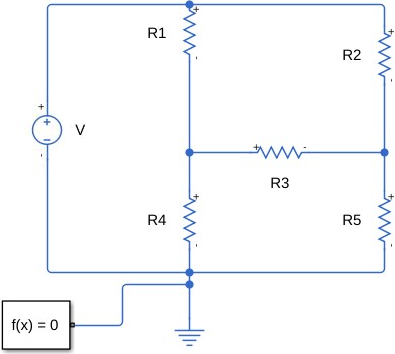
\includegraphics[width=0.5\linewidth]{fig/lab1circuitmatlab.png}
  \caption{Circuito recreado no Matlab}
  \label{fig:circuit-simulink}
\end{figure}

Inicialmente, o circuito foi remontado no Simulink de forma a refletir fielmente
o arranjo teórico. Foram utilizados componentes eletrônicos como resistores,
fontes de tensão e referência elétrica, todos configurados de acordo com os
parâmetros estabelecidos. A Figura~\ref{fig:circuit-simulink} apresenta a
montagem do circuito no ambiente de simulação.

\begin{figure}[H]
  \centering
  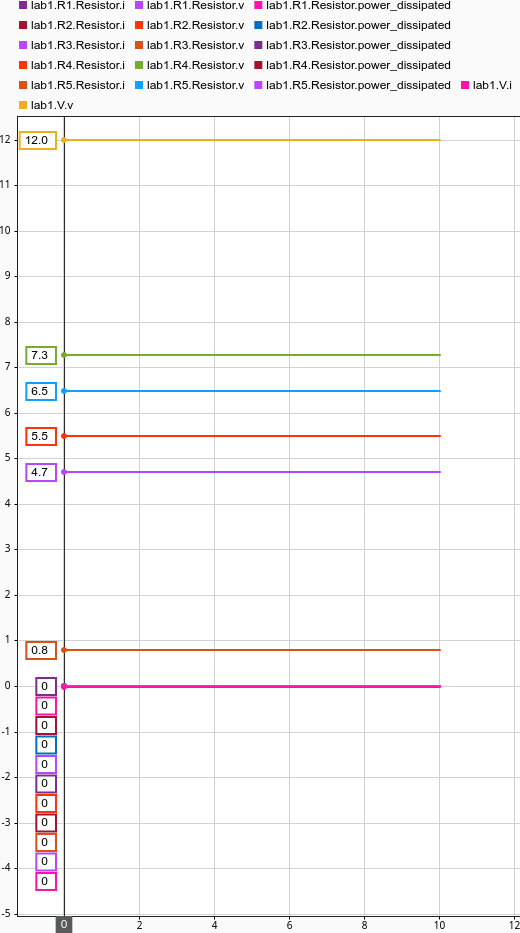
\includegraphics[width=0.7\linewidth]{fig/lab1results.png}
  \caption{Resultados apresentados pelo Matlab}
  \label{fig:simulink-results}
\end{figure}

Após a simulação, os resultados obtidos para as tensões, correntes e potências
nos diversos elementos do circuito foram registrados, conforme ilustrado na
Figura~\ref{fig:simulink-results}. Esses valores foram posteriormente
organizados em tabelas comparativas com os dados teóricos e os dados obtidos em
medições reais. A boa concordância entre os resultados simulados e teóricos
reforça a consistência da análise e evidencia a confiabilidade da simulação como
ferramenta de apoio ao estudo de circuitos elétricos, além da assertividade da
análise realizada por nós.
\section{Experimento Laboratorial}

Nesta etapa, o circuito proposto foi montado fisicamente em bancada utilizando
componentes reais disponíveis no laboratório.

\begin{figure}[H]
  \centering
  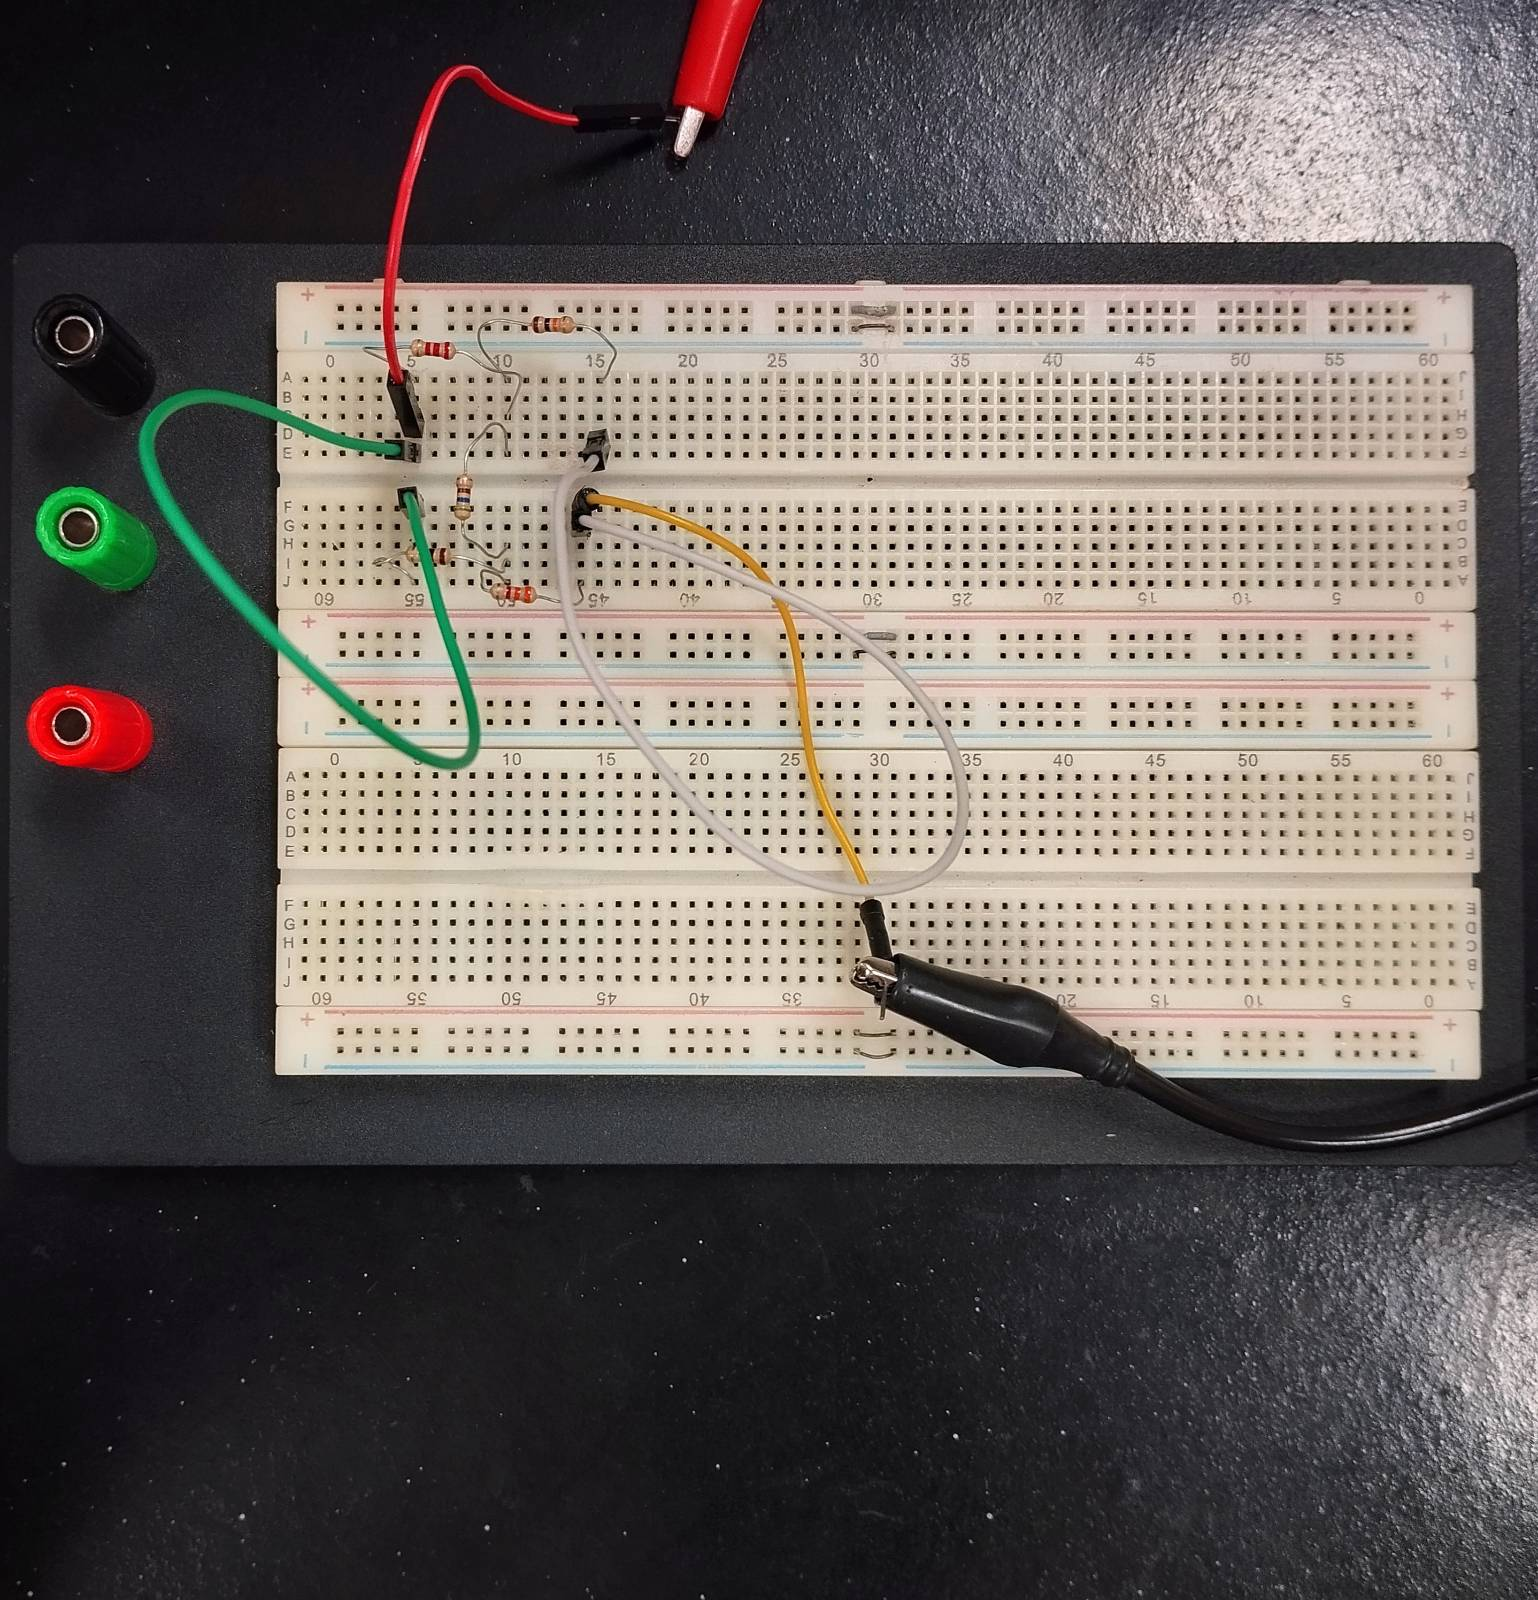
\includegraphics[width=0.5\linewidth]{fig/lab1realcircuit.jpeg}
  \caption{Circuito montado em laboratório}
  \label{fig:real-circuit}
\end{figure}

\begin{figure}[H]
  \centering
  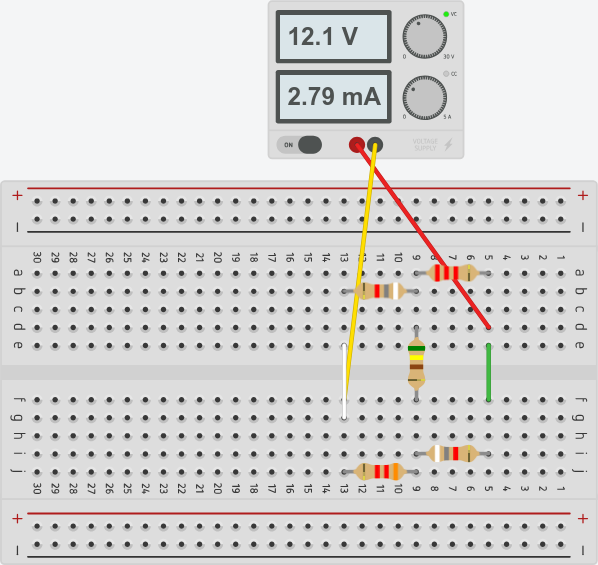
\includegraphics[width=0.5\linewidth]{fig/lab1tinkercad.png}
  \caption{Circuito recreado no Tinkercad para melhor visualização}
  \label{fig:tinkercad}
\end{figure}

Ao realizar medições com multímetros de bancada, foram observadas variações nos
valores nominais dos componentes, como apresentado a seguir:

\begin{itemize}
  \item Fonte: \(V = \SI{12.01}{\volt} \neq \SI{12}{\volt}\)
  \item \(R_1 = \SI{2.15}{k\ohm} \neq \SI{2.2}{k\ohm}\)
  \item \(R_2 = \SI{9.78}{k\ohm} \neq \SI{10}{k\ohm}\)
  \item \(R_3 = \SI{540}{\ohm} \neq \SI{560}{\ohm}\)
  \item \(R_4 = \SI{9.83}{k\ohm} \neq \SI{10}{k\ohm}\)
  \item \(R_5 = \SI{3.20}{k\ohm} \neq \SI{3.3}{k\ohm}\)
\end{itemize}

Estas discrepâncias entre os valores reais e ideais são esperadas em contextos
experimentais. Elas resultam de fatores como:

\begin{itemize}
  \item Tolerância dos componentes, geralmente indicada no corpo dos resistores
  (por exemplo, 5\% ou 1\%);
  \item Variações na tensão de alimentação, especialmente se a fonte não for
  regulada com precisão;
  \item Influências ambientais como temperatura e umidade, que podem afetar
  levemente a resistência elétrica.
\end{itemize}

As tensões e correntes em cada resistor e na fonte foram medidas em laboratório e serão apresentadas na seção de Resultados (\ref{sec:resultados}).
\section{Resultados}\label{sec:resultados}

Nesta seção, são apresentados os resultados obtidos nas etapas de análise
teórica, simulação computacional e medição prática do circuito proposto. A
comparação entre os três métodos permite avaliar a consistência dos conceitos
aplicados, a precisão dos modelos simulados e o comportamento real dos
componentes em laboratório. As tabelas a seguir organizam os dados de tensão,
corrente e potência para cada elemento do circuito, destacando eventuais
discrepâncias e reforçando a importância da análise crítica dos resultados
experimentais.

\begin{table}[H]
\centering
\begin{tabularx}{0.9\textwidth}{l *{7}{>{\centering\arraybackslash}X}}
\textbf{Elemento} & \multicolumn{2}{c}{\textbf{Resultado Teórico}} & \multicolumn{2}{c}{\textbf{Resultado Simulado}} & \multicolumn{2}{c}{\textbf{Resultado Real}} \\
 & Tensão (V) & Corrente (mA) & Tensão (V) & Corrente (mA) & Tensão (V) & Corrente (mA) \\
\hline
Fonte & 12.00 & 2.69  & 12.00  & 2.695  & 12.01 & 2.68  \\
R1    & 4.70  & 2.1   & 4.717  & 2.144  & 4.73  & 2.1 \\
R2    & 5.49  & 0.54  & 5.510  & 0.551  & 5.54  & 0.5 \\
R3    & 0.79  & 1.41  & 0.793  & 1.416  & 0.79  & 1.3 \\
R4    & 7.28  & 0.72  & 7.283  & 0.728  & 7.27  & 0.6 \\
R5    & 6.51  & 1.97  & 6.490  & 1.967  & 6.46  & 1.9 \\
\end{tabularx}
\caption{Comparação dos resultados teóricos, simulados e reais dos elementos do circuito}
\end{table}

\begin{table}[H]
\centering
\begin{tabularx}{0.7\textwidth}{lXXX}
\textbf{Elemento} & \textbf{Potência Teórica (mW)} & \textbf{Potência Simulada (mW)} & \textbf{Potência Real (mW)} \\
\hline
Fonte & 32.28 & 32.291 & 32.187 \\
R1    & 10.06 & 10.113 & 9.933  \\
R2    & 3.01  & 3.036  & 2.77   \\
R3    & 1.11  & 1.122  & 1.027  \\
R4    & 5.29  & 5.304  & 4.362  \\
R5    & 12.82 & 12.765 & 12.274 \\
\end{tabularx}
\caption{Comparação de potência dissipada nos resistores do circuito}
\end{table}
\newpage
\section{Análise dos Resultados}

Após realizar análises nas três modalidades, teórica, simulado e experimental, verificamos que os valores calculados entre si são bem próximos ou idênticos, o que serve como um grande indicativo que os nossos resultados são coerentes, contudo ao investigar as discrepâncias entre os valores obtidos, é possível observar alguns motivos pelo ocorrido. 

Primeiramente, como já apontado na secção do experimento laboratorial, os resistores tem um nível de tolerância pelo qual pode variar sua resistência, isso por si só já implicaria numa diferença nas tensões e correntes do circuito dos experimento real, comparado com os cálculos teóricos e a simulação. Investigando mais a frente, podemos conferir que tanto os cálculos teóricos realizados quanto o modelo de simulação utilizado no \(MATLAB\) foram feitos sobre a consideração de que o circuito utilizado como objeto de estudo era ideal ou perfeito, isto é, seus resistores têm valor exato e sem tolerância, fontes de tensão/corrente são perfeitas com nenhuma resistência internas e fios e conexões têm resistência e indutância desprezíveis, o que não acontece num experimento real, onde todas essas limitações físicas inevitavelmente afetam a medição das grandezas de um circuito elétrico.

Além das diferenças derivadas de natureza física do circuito elétrico, existe também um ponto a ser levantando que é o dos métodos numéricos utilizados, que pode ser observado não só em contrasto com o experimento real mas também o teórico e simulado, pois ao realizar a análise nodal foi feito diversas aproximações e trucamentos para viabilizar e facilitar os cálculos, enquanto o modelo matemático do \(MATLAB\) também, apesar de ser muito mais preciso, utiliza métodos como erros de discretização e arredondamentos numéricos como limitações da precisão de ponto flutuante, que pode alterar com certo nível de precisão, os valores esperados de até mesmo um sistema ideal. 

E por fim, temos também as varáveis do ambiente onde se foi executado o experimento real, como instrumentos de medição (multímetros, osciloscópios) que têm precisão limitada, ruídos eletromagnéticos que podem interferir nas medidas e variações térmicas, pois resistores mudam de valor de acordo com a temperatura.
\section{Conclusão}

Podemos concluir que uma simulação computacional do circuito é útil para análise teórico mas ignora imperfeições do mundo real, enquanto o experimento em laboratório revela efeitos práticos (tolerâncias, ruído, etc), mas exige cuidado com medições e calibração, mas que ambos são ferramentas confiáveis de desenvolvimento do estudo de circuitos elétricos e que o resultado de ambos coincidiram, com certa taxa de variação, com os resultados teóricos esperados. Conferimos que seja adequado usar a simulação para validar o conceito, mas sempre ajustar o projeto com testes reais, considerando tolerâncias e efeitos não ideais.

\newpage

\printbibliography[title=Referências]

\end{document}
